
\chapter{\IfLanguageName{dutch}{Stand van zaken}{State of the art}}
\label{ch:stand-van-zaken}
In dit hoofdstuk worden de verschillen tussen een informationeel en operationeel netwerk uitvoerig besproken. Dit zijn antwoorden op enkele deelvragen die te vinden zijn in sectie~\ref{subsec:deelonderzoeksvraag}. Daarnaast wordt de convergentie van beide netwerken besproken alsook de voor- en nadelen.
\section{\IfLanguageName{dutch}{Informatie technologie}{Informatie technologie}}
\label{sec:Informatie technologie}
\subsection{\IfLanguageName{dutch}{Definitie Informatie technologie}{Definitie Informatie technologie}}
\label{subsec:Definitie Informatie technologie}
Volgens~\textcite{Castagna2021} is IT (informationele technologie) het gebruik van computers, opslag, netwerken, infrastructuur, processen en andere fysieke apparaten om alle vormen van elektronische gegevens te creëren, verwerken, op te slaan, beveiligen en uit te wisselen. 

IT is vrij nieuw als we kijken naar de geschiedenis van bedrijven. Sinds dat de computer bestaat en internet er is, zijn processen in een bedrijf afhankelijker geworden van IT, waaronder besluitvorming en strategie, samenwerking, verkoop en klantenservice~\autocite{SecureiconTeam2019}. Er zijn enkele cruciale IT-componenten waar een organisatie de dag van vandaag gebruik van maakt, zie figuur~\ref{fig:2.1}.


\begin{figure}
    \includegraphics[width=\textwidth]{definitie IT}
    \caption{Componenten van een IT netwerk\autocite{Castagna2021} \label{fig:2.1}} 
\end{figure}

Zoals te zien is in figuur~\ref{fig:2.1} zijn er heel wat componenten in een IT-organisatie. Wij zullen ons in deze thesis beperken tot de belangrijkste componenten in de IT-omgeving. 
\begin{itemize}
    \item Bestandsserver
    \item Applicatieserver
    \item Webserver
    \item Mailserver
    \item DHCP-server
    \item DNS-server
    \item Software
\end{itemize}
\subsection{\IfLanguageName{dutch}{Componenten}{Componenten}}
\label{subsec:ITcomponenten}
\subsubsection{\IfLanguageName{dutch}{Bestandsserver}{Bestandsserver}}
\label{subsubsec:Bestandsserver}
Een bestandsserver, ook wel~\footnote{FTP-server staat voor file transfer protocol server en wordt gebruikt voor de uitwisseling van bestanden tussen computers}FTP-server genoemd, is een centrale server in het netwerk van een organisatie die bestanden ter beschikking stelt aan aangesloten gebruikers. Het is een centrale opslagplaats die interne gebruikers de kans geeft om bestanden met elkaar te delen. De serverbeheerder kan specifieke regels gebruiken, zodat niet elke gebruiker aan alle bestanden kan. Hij kan ervoor zorgen dat enkele gebruikers enkel de bestanden kunnen bekijken en niet aanpassen, dat ze niets in een map kunnen plaatsen en kan vele andere regels instellen. Bestandsservers kunnen ook geconnecteerd worden met het internet, dit zorgt ervoor dat personeel makkelijk van thuis de nodige bestanden kan gebruiken. Uitwisseling van bestanden is niet de enige functie van een bestandsserver, de servers worden ook vaak gebruikt als opslagplaats voor programma's die toegankelijk moeten zijn voor meerdere netwerkgebruikers, en als back-upserver~\autocite{Ionos2019}.

Bestandsservers hebben een hoge capaciteit aan opslagplaats, werkgeheugen en processorkracht nodig om goed te functioneren. Deze capaciteit hangt af van de hoeveelheid bestanden en gebruikers er aanwezig zijn binnen de omgeving. Toegang tot de server via het lokaal netwerk kan via het SMB (server message block) protocol. Om toegang te krijgen via het internet wordt er gebruik gemaakt van het FTP (file transfer protocol) protocol of SFTP (secure FTP) protocol~\autocite{Ionos2019}.

Een bestandsserver heeft vele voordelen voor een bedrijf. Het eerste voordeel is de centraliteit die ervoor zorgt dat geautoriseerde gebruikers toegang hebben tot opgeslagen bestanden. Dit zorgt ervoor dat van op afstand werken gemakkelijker is. Ongewenste acties zoals het verwijderen van bestanden kunnen worden uitgesloten door een goede configuratie van het systeem. Er kan ook makkelijk worden gewerkt met dezelfde versie aangezien ze elke verandering van een document zien. Als er geen centrale server zou zijn, zouden ze alles moeten delen of via verwisselbare media moeten verzenden wat heel tijdrovend is. Het tweede voordeel is dat bestandsservers de druk op gebruikers vermindert. Alle bedrijfsdocumenten en back-ups kunnen op de bestandsserver worden opgeslagen. Als de organisatie de juiste structuur gebruikt is de gehele bestandsinventaris veel overzichtelijker. Ten laatste is er de toegankelijkheid via het internet. Het maakt het mogelijk om overal aan de bestanden aan te kunnen. Het is verschillend van een cloudtoepassing, omdat het bedrijf met een eigen server alle controle houdt over de bestanden en de beveiliging~\autocite{Ionos2019}.

\subsubsection{\IfLanguageName{dutch}{Applicatieserver}{Applicatieserver}}
\label{subsubsec:Applicatieserver}
Volgens~\textcite{TechTerms2019} en~\textcite{ProTeam2018} is een applicatieserver een mix van hardware en software componenten waarmee zowel webapplicaties kunnen worden gemaakt als een serveromgeving om deze uit te voeren. Een applicatieserver is ontworpen om applicaties en bijbehorende diensten te installeren, te bedienen en te hosten voor eindgebruikers, IT-diensten en organisaties. Een ander voordeel van een applicatieserver is dat het de hosting en levering van bedrijfstoepassingen vergemakkelijkt. Afhankelijk van wat er wordt geïnstalleerd kan een applicatieserver ingedeeld worden als: webserver, databasetoepassingserver, toepassingsserver voor algemene doeleinden of bedrijfstoepassingsserver. Applicatieservers kunnen een eigen interface hebben via computers, maar ze kunnen ook zorgen voor hun eigen hulpbronnen, evenals voor transactieverwerking, berichtenverkeer en het uitvoeren van beveiligingstaken. Voor high-end eisen hebben applicatieservers meestal een hoge beschikbaarheid, clustering, load-balancing en een geïntegreerde redundantie. 

Applicatieservers worden het best gebruikt wanneer er een integratie is met databanken en servers, bijvoorbeeld webservers, die reeds in de IT-infrastructuur van de organisatie staan. Een belangrijke reden hiervoor is dat een applicatieserver kan dienen als middel om de integriteit van code en gegevens te waarborgen door middel van een geïntegreerde en gecentraliseerde aanpak voor het bijwerken en actualiseren van toepassingen. Als dit ontbreekt, is er een grote kans dat er verschillende versies van dezelfde applicatie in het bedrijf zijn. Een andere belangrijke reden om een applicatieserver in een IT-omgeving te plaatsen is voor een extra beveiligingslaag. Als er een applicatielaag tussen de webserver en de databank wordt geplaatst zijn aanvallen zoals een ~\footnote{Een SQL-injectie is een type kwetsbaarheid van computerapplicaties, meestal webapplicaties. Applicaties maken meestal gebruik van een databank om data op te slaan. Hackers proberen een SQL-statement als invoer om de gehele databank te doen falen.}SQL-injectie niet mogelijk. De beveiliging wordt verder versterkt door authenticatieprocessen en toegangsbeheer. Als laatste zorgt een applicatieserver voor meer controle over het netwerkverkeer~\autocite{ProTeam2018}. 

Op het eerste zicht lijken een applicatieserver en een webserver heel goed op elkaar, toch zijn er enkele verschillen. Een applicatieserver houdt zich bezig met het aanbieden van bedrijfslogica aan applicaties via een reeks protocollen. Een webserver werkt met HTTP-verzoeken, beantwoordt en verwerkt deze om websitefunties uit te voeren en host de website. Normaal maakt een webserver geen gebruik van transacties of databank connecties, maar het kan wel voorzien zijn van clustering, caching en load-balancing~\autocite{ProTeam2018}.

\subsubsection{\IfLanguageName{dutch}{Webserver}{Webserver}}
\label{subsubsec:Webserver}
Een webserver is software en hardware die samenwerkt. Aan de hardware kant is een webserver een computer dat webserver software opslaat en een website bestand bevat. Dit website bestand is meestal opgemaakt uit html, css en javascript. Aan de software kant is een webserver een verzameling van taken die ervoor zorgen dat gebruikers aan de website kunnen. Dit is minimum een HTTP-server. Een HTTP-server is software dat URL's kan vertalen naar de webserver. Als een browser een bestand nodig heeft op een webserver, zal de browser een HTTP request sturen. Wanneer de request naar de juiste webserver gaat, zal de software een HTTP-accept terug sturen, zodat het een pagina kan laden, de functionaliteit van een statische webserver kun je zien op figuur~\ref{fig:2.2}~\autocite{MDN2021}. 
\begin{figure}
    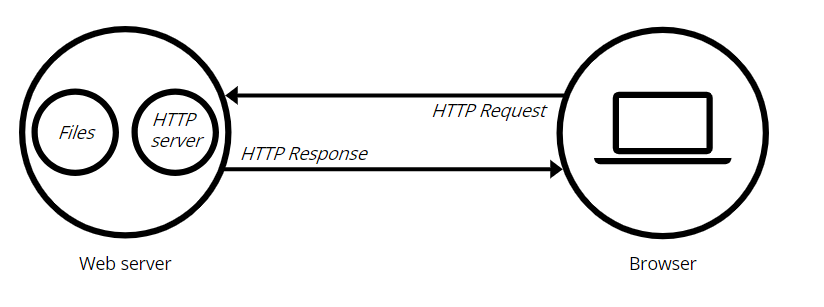
\includegraphics[width=\textwidth]{Webserver}
    \caption{Statische webserver funcionaliteit\autocite{MDN2021} \label{fig:2.2}} 
\end{figure}

Er zijn 2 soorten webservers. Als eerste is er de statische webserver. Deze bestaat uit een computer met een HTTP-software. Het wordt statisch genoemd, omdat de server de bestanden naar je browser stuurt zoals ze zijn. Als tweede is er een dynamische webserver. Een dynamische webserver bestaat uit een statische webserver plus extra software, meestal een applicatieserver en een databank. Het wordt een dynamische webserver genoemd, omdat de applicatieserver de gehoste bestanden aanpast voordat de inhoud via HTTP naar een browser wordt gestuurd. Een voorbeeld van een dynamische webserver is Wikipedia. Wikipedia bestaat uit een paar HTML-templates die worden gevuld met de gigantische databank van informatie dat ze hebben. Dit is eenvoudiger om de inhoud te onderhouden dan altijd een nieuwe statische HTML-pagina te moeten maken. De functionaliteit van een dynamische webserver zie je in figuur~\ref{fig:2.3}~\autocite{MDN2021}.
\begin{figure}
    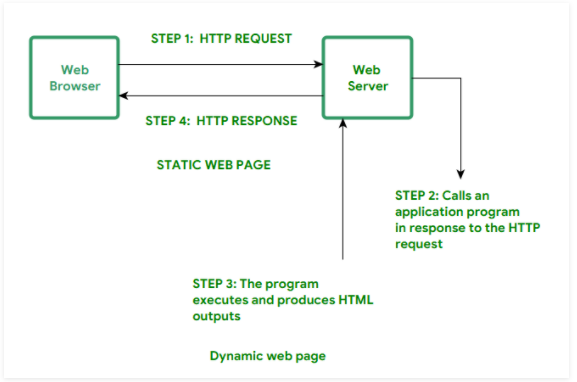
\includegraphics[width=\textwidth]{Webserver dynamic}
    \caption{Dynamische webserver funcionaliteit\autocite{GeeksforGeeks2020} \label{fig:2.3}}
\end{figure}
\subsubsection{\IfLanguageName{dutch}{Mailserver}{Mailserver}}
\label{subsubsec:Mailserver}
Een mailserver is een machine of toepassing verantwoordelijk voor het afhandelen van berichten en is vergelijkbaar met een postdienst. De functie van een mailserver is het ontvangen en afleveren van e-mails. Wanneer een mail verstuurd wordt,gaat het gewoonlijk door een reeks van e-mailservers totdat de ontvanger bereikt is. Het proces is heel snel en efficiënt, maar er zit veel complexiteit achter het verzenden en ontvangen van e-mails~\autocite{Gatefy2021}.

We kunnen een e-mailserver opdelen in 2 soorten, namelijk uitgaande en inkomende servers. Uitgaande e-mailservers worden SMTP-servers (Simple Mail Transfer Protocol) genoemd en inkomende worden POP3(Post Office Protocol) en IMAP(Internet Message Access Protocol) servers genoemd. Het verschil tussen POP3 en IMAP is de ruimte waar de berichten worden opgeslagen. Bij POP3 worden berichten meestal op het apparaat opgeslagen en bij IMAP op de server zelf. Over het algemeen is een IMAP-server complexer en flexibeler dan POP3. E-mails verzenden via een POP3 of IMAP-server gebeurt in 4 stappen~\autocite{Gatefy2021}:
\begin{itemize}
    \item Stap 1: verbinding maken met de SMTP-server. Wanneer een mail verstuurd wordt,maakt de e-mailservice zoals gmail en outlook verbinding met de SMTP-server. Deze SMTP-server is verbonden met het domein en heeft een specifiek adres. Tijdens deze stap zal de maildienst de SMTP-server voorzien van informatie zoals uw e-mailadres, de inhoud van het bericht en het e-mailadres van de ontvanger.
    \item Stap 2: Verwerking van het e-maildomein van de ontvanger. De SMTP-server zal het e-mailadres van de ontvanger moeten identificeren en verwerken. Als het een e-mail is naar een ontvanger gaat het rechtstreeks naar de IMAP of POP3 server. Als het naar een e-mailadres gaat van een ander bedrijf moet de SMTP-server communiceren met de e-mailserver van dat bedrijf. 
    \item Stap 3: identificeren van het IP-adres van de ontvanger. Hier zal de SMTP-server communiceren met de DNS-server (Domain Name System) om de server van de ontvanger te vinden. Dns zal het domein omzetten naar een IP-adres dat een machine of server identificeert die verbonden is met het internet. Zo kan de SMTP-server het bericht naar de juiste server sturen.
    \item Stap 4: de e-mail afleveren. Nadat de e-mail langs veel niet-gerelateerde SMTP-servers is gegaan zou het tot de SMTP-server van de ontvanger moeten geraakt zijn. Wanneer dit het geval is, zal de SMTP het bericht controleren en doorsturen naar de IMAP of POP3-server. De e-mail komt dan in een wachtrij terecht tot  hij beschikbaar is voor de ontvanger. 
\end{itemize}

E-mailservers moeten beschermd worden. Veel cyberaanvallen vinden plaats via e-mails. Phishing is hier een voorbeeld van. Dit is een soort van internetfraude dat bestaat uit het oplichten van mensen door ze te lokken naar een valse website. Er worden veel valse mails verstuurd en de gebruikers moeten zich daar bewust van zijn~\autocite{Gatefy2021}.
 
\subsubsection{\IfLanguageName{dutch}{DHCP-server}{DHCP-server}}
\label{subsubsec:DHCP-server}
DHCP staat voor dynamic host configuration protocol en is een netwerk protocol dat wordt gebruikt in IP-netwerken. De DHCP-server voorziet componenten in het netwerk van een IP-adres en andere informatie met betrekking tot het netwerk, zodat al deze toestellen kunnen communiceren met elkaar. DHCP geeft naast IP-adressen ook een subnet mask, default gateway adres, DNS-adres en andere configuratie parameters mee. De voornaamste reden waarom DHCP gebruikt wordt, is het beheer van IP- adressen op het netwerk. DHCP kan 2 toestellen niet hetzelfde IP-adres geven wat wel zou kunnen voorkomen als je ze statisch instelt. De meeste gebruikers weten ook niet wat een IP-adres is, wat ervoor zorgt dat statisch instellen moeilijk is~\autocite{Kerravala2018}.

DHCP vereist enkele componenten~\autocite{Kerravala2018}:
 \begin{itemize}
     \item DHCP-server: dit is het toestel dat de DHCP-service bezit. Deze zal alle informatie omtrent het netwerk uitdelen. Een router of een server wordt hiervoor gebruikt.
     \item DHCP-client: dit is een toestel dat configuratie informatie nodig heeft van een DHCP-server. Dit kan een computer, telefoon, IoT toestel of een ander toestel zijn dat verbonden is met het internet. De meeste toestellen zijn geconfigureerd dat ze automatisch DHCP-informatie verkrijgen.
     \item IP-adres pool: dit is de range van adressen dat een DHCP-server kan uitdelen aan gebruikers.
     \item Subnet: een netwerk kan worden ingedeeld in subnetwerken, zodat alle groepen makkelijk zichtbaar zijn.
     \item Lease: De tijd dat een DHCP-client de informatie bijhoudt. Als de lease overtreden wordt, zal de client alle nodige informatie+ vernieuwen.
     \item DHCP-relay: dit zijn servers in het subnet die DHCP-requests doorsturen naar de geconfigureerde DHCP-server. De server zal antwoorden terug sturen naar de DHCP-relay die ze doorstuurt naar de clients. Dit zorgt ervoor dat één DHCP-server kan gebruikt worden in meerdere subnetten.
 \end{itemize}

Een DHCP heeft niet als enige voordeel om het management simpeler te maken. Enkele andere voordelen zijn~\autocite{Kerravala2018}:
\begin{itemize}
    \item Exacte IP configuratie/geen conflict met andere toestellen: de adressen die worden uitgedeeld zullen exact zijn, twee keer hetzelfde adres verkrijgen zal niet lukken en typfouten kunnen ook niet gemaakt worden.
    \item Automatisatie: doordat DHCP elk toestel automatisch een adres aanlevert moet er niet een persoon worden ingezet om dit allemaal te regelen. Alle toestellen voorzien van een IP-adres en alles bijhouden is heel tijdrovend. 
    \item Verandering: als het bedrijf beslist om de range aan te passen zal de DHCP-server elk toestel dat verbonden is een ander IP-adres geven. Zo moet niet elk toestel apart worden aangepast.
\end{itemize}

Naast alle voordelen die DHCP biedt moet er ook worden nagedacht over de veiligheid. Het DHCP-protocol heeft geen authenticatie nodig, dit zorgt voor veiligheidsrisico's zoals: IP-adresuitputting door aanvallen en clients die niet geautoriseerd zijn om een IP-adres te krijgen. Aangezien clients geen manier hebben om een DHCP-server te valideren kan het zijn dat malafide servers worden gebruikt, wat kan leiden tot~\footnote{Een denial-of-service aanval wordt gebruikt om machines of netwerken onbeschikbaar te maken.}denial-of-service aanvallen of~\footnote{Een man-in-the-middle aanval is een aanval waarbij informatie tussen 2 partijen wordt onderschept zonder dat beide partijen daar weet van hebben.}man-in-the-middle aanvallen waarbij een valse server gegevens onderschept. Omgekeerd valideert de DHCP-server de clients ook niet. Dit zorgt ervoor dat elk toestel dat een verzoek indient ook een adres krijgt. Een hacker kan zo een computer instellen om altijd een nieuw adres te vragen, zodat de adressen uitgeput worden~\autocite{Kerravala2018}.
\subsubsection{\IfLanguageName{dutch}{DNS-server}{DNS-server}}
\label{subsubsec:DNS-server}
Een DNS(Domain Name System) is een server dat een website adres vertaalt naar een IP-adres. Zonder een DNS-server zou het onmogelijk zijn om via een web browser een website te vinden. Je kunt het vergelijken met een telefoonboek. Wanneer iemand een website opzoekt, zal de server het IP-adres zoeken van die website. Deze combinatie van IP-adressen en bijhorende namen kunnen niet op één server worden opgeslagen. In plaats daarvan zijn er heel veel DNS-servers die alles opslaan. Elke computer die een adres moet weten kan dit aan zijn DNS-server vragen die kan communiceren met andere DNS-servers~\autocite{Johnson2021}. 

Binnen DNS wordt er gebruikt gemaakt van 4 servers. De Resolving name server, root name server en TLD name server zijn recursieve servers, omdat ze geen antwoord bevatten maar de vraag doorsturen naar een andere server~\autocite{Petters2021}.
\begin{itemize}
    \item Resolving name server: dit is de server die antwoordt op een DNS-query. Het zal aan andere DNS-servers vragen voor het adres als dit niet in zijn cache opgeslagen is.
    \item Root name server: deze server geeft top level domain servers terug aan de resolving name server. Enkele voorbeelden hiervan zijn: .com, .be, .vlaanderen en vele andere.
    \item TLD name server: dit is de server die aanduidt bij welke authoritative name server de juiste informatie staat die nodig is.
    \item Authoritative name server: dit is de laatste stop bij een DNS-query. Deze server bezit het IP-adres van de desbetreffende naam.
\end{itemize} 


Een DNS-query wordt uitgevoerd in 6 stappen:
\begin{itemize}
    \item Een DNS-query start bij het opzoeken van een website. 
    \item Er zal worden gekeken of de website in de lokale cache staat. Als dit niet het geval is, zal het kijken naar de cache van de resolving name server.
    \item De resolving name server zal een vraag sturen naar de root name server. Deze zal antwoorden met een TLD name server voor het gevonden domein.
    \item De resolving name server kan hierna een vraag sturen naar de TLD name server. Deze zal als antwoord een authoritative name server terugsturen.
    \item De resolving name server zal de vraag stellen aan de authoritative name server. Deze server zal het IP-adres terugsturen naar de resolving name server.
    \item De resolving name server staat in contact met de computer en zal het adres kunnen afleveren. 
    \end{itemize}


\subsubsection{\IfLanguageName{dutch}{Software}{Software}}
\label{subsubsec:Software}
Volgens~\textcite{Castagna2021} zijn er 2 categorieën van software. Enerzijds is er de software die systemen nodig hebben (systeem software), anderzijds zijn er de applicaties die draaien op deze systemen. Systeem software omvat de programma's die zorgen voor de basisfuncties van het computer beheer.
\begin{itemize}
    \item Besturingssystemen.
    \item Basis input/output systemen (BIOS).
    \item Boot programma's.
    \item Drivers.
\end{itemize} 
Applicatie's zijn software die worden geïnstalleerd voor eindgebruikers en die het makkelijk maken om verschillende taken uit te voeren.
\begin{itemize}
    \item databanken.
    \item e-mail servers.
    \item ERP systemen.
    \item Transactie systemen.
\end{itemize}

\subsection{\IfLanguageName{dutch}{IT-protocollen}{IT-protocollen}}
\label{subsec:IT protocollen}
Volgens~\textcite{Sharon2019} en~\textcite{Subham2021} gebruiken computers protocollen om informatie met elkaar te delen via een netwerk. Eerst was communicatie moeilijker tussen computers omdat elke verkoper zijn eigen manier had van communiceren tussen zijn eigen computers. Dit zorgde ervoor dat communicatie tussen computers van andere verkopers niet mogelijk was. Het werd snel duidelijk dat er een standaard nodig was waarmee computers van alle verkopers met elkaar konden communiceren. Deze standaard is TCP/IP en zal verder uitgelegd worden. Andere protocollen die veel worden gebruikt binnen een IT-omgeving zijn:
\begin{itemize}
    \item ICMP (internet control message protocol)
    \item ARP (address resolution protocol)
    \item UDP (user datagram protocol)
    \item HTTP (hypertext transfer protocol)
    \item DHCP (dynamic host configuration protocol)
    \item STP (spanning tree protocol)
    \item FTP (file transfer protocol)
    \item SSH (secure shell protocol)
    \item SFTP (ssh file transfer protocol)
\end{itemize}

\subsubsection{\IfLanguageName{dutch}{TCP/IP}{TCP/IP}}
\label{subsec:TCP/IP}
TCP en IP zijn twee verschillende protocollen. IP is het deel dat het adres krijgt waarnaar gegevens moeten verzonden worden en TCP is verantwoordelijk voor het leveren van de data zodra het adres gekend is. Het is niet nodig om een verschil te maken tussen beide aangezien ze vaak samen worden gebruikt~\autocite{Sharon2019}. 

TCP/IP werd ontwikkeld door het Amerikaanse Ministerie van defensie om te specificeren hoe computers gegevens moesten overbrengen naar elkaar. TCP/IP legt veel nadruk op nauwkeurigheid en heeft verschillende stappen om ervoor te zorgen dat gegevens correct worden verzonden tussen twee computers. Als TCP/IP een bericht in één stuk zou versturen en er treed een probleem op dan zou dit hele bericht opnieuw moeten verzonden worden. TCP/IP verdeelt daarom zijn berichten in verschillende pakketen bij het verzenden van data. Elk pakket kan een andere route nemen als de eerste route niet beschikbaar of overbelast is. TCP/IP verdeelt de verschillende taken voor communicatie in enkele lagen. Elke laag heeft een andere functie. De data gaat door 4 afzondelijke lagen voordat de data verstuurt wordt en zal vervolgens in omgekeerde volgorde de data terug samenstellen. Het doel van deze lagen is om alles gestandaardiseerd te houden. Elke leverancier gebruikt dezelfde lagen, zodat elk component kan communiceren met andere componenten~\autocite{Sharon2019}. 

De vier lagen waarvan het TCP/IP-protocol gebruik maakt zijn de datalinklaag, internetlaag, transportlaag en applicatielaag. De datalinklaag staat in voor de fysieke onderdelen voor het verzenden en ontvangen van gegevens. Dit gebeurt via een ethernet-kabel, het draadloze netwerk, de netwerkinterfacekaart, het stuurprogramma van de computer en dergelijke. De internetlaag zorgt voor de verplaatsing van de pakketten over het internet. De transportlaag staat in voor een betrouwbare gegevensverbinding tussen apparaten. Het verdeelt de data in pakketten, bevestigt de pakketten die het van het andere apparaat heeft ontvangen en zorgt ervoor dat het andere apparaat de ontvangen pakketten bevestigt. Als laatste is er de toepassingslaag. Dit is een groep toepassingen die netwerkcommunicatie vereisen. Een voorbeeld van de toepassingslaag zijn e-mails. Aangezien de lagere lagen de details van de communicatie afhandelen, hoeven de toepassingen zich hier niet mee bezig houden~\autocite{Sharon2019}. 


\subsection{\IfLanguageName{dutch}{IT-security}{IT-security}}
\label{subsec:IT security}
\subsubsection{\IfLanguageName{dutch}{Wat valt er onder IT-security?}{Wat valt er onder IT-security?}}
\label{subsec:Wat valt er onder IT security?}
Volgens~\textcite{Kieron2020} verwijst IT-beveiliging naar de bescherming van digitale gegevens binnen een IT-infrastructuur en het veiligheidsonderhoud van de computersystemen en netwerken waarop deze gegevens worden bijgehouden. De term IT-beveiliging wordt gebruikt om internet en externe bedreigingen te beschrijven. Ook dekt de term strategieën die worden ingezet om digitale gegevens te beschermen tegen aanvallen op elk punt van de infrastructuur. 

Sinds dat het internet bestaat zijn er hackers die proberen data van grote bedrijven te stelen. Als ze deze data in handen krijgen kunnen ze hier grote geldsommen voor vragen. Cybercriminelen kunnen op allerlei manieren gebruik maken van de IT-netwerken en de technieken die ze gebruiken worden alsmaar moeilijker. Enkele cyberaanvallen die vandaag de dag veel worden gebruikt zijn:
\begin{itemize}
    \item ~\footnote{Malware is elke software dat wordt gebruikt om computersystemen te hinderen.}Malware
    \item ~\footnote{Phishing is een vorm van internetfraude waarbij mensen worden gelokt naar een valse site.}Phishing
    \item Man-in-the-middle aanval
    \item Denial-of-service aanval
    \item SQL-injectie
    \item ~\footnote{Een zero day aanval is een aanval die misbruik makat van de zwakke onbekende delen van software.}Zero day aanval
\end{itemize}
Naast al deze externe aanvallen moet er ook rekening gehouden worden met interne bedreigingen. Dit betekent dat databanken moeten beschermd worden van alle personeelsleden die hier geen toegang voor hebben en dat potentiële dieven geen toegang hebben tot vertrouwelijke gegevens. Aangezien het bedreigingslandschap zo groot is kan geen enkele beveiligingsmaatregel elke bedreiging wegnemen. Daarom zijn er een verschillende types van beveiliging die samenwerken om de gegevens van een organisatie zo goed mogelij te beschermen tegen aanvallen, ongeacht waar of hoe de aanval plaatsvindt. Deze types van beveiliging zijn: netwerkbeveiliging, internetbeveiliging, applicatiebeveiliging, endpointbeveiliging en cloudbeveiliging~\autocite{Kieron2020}. 

Netwerkbeveiliging wordt gebruikt om kwaadwillende gebruikers of onbevoegden geen toegang te geven tot het netwerk. Het zorgt ervoor dat de bruikbaarheid, betrouwbaarheid en integriteit van de data wordt bewaard. Deze vorm van beveiliging is een must om te voorkomen dat hackers toegang krijgen tot gegevens in het netwerk. Netwerkbeveiliging wordt steeds meer een grotere uitdaging, dit komt omdat veel bedrijven uitbreiden qua toestellen en migreren naar de cloud~\autocite{Cisco}.

Internetbeveiliging ook wel cybersecurity genoemd is een term die betrekking heeft op de bescherming van alle gegevens die via het internet worden verzonden of ontvangen. Het doel is om de online bedreigingen te verminderen. Beveiligingssoftware, zoals een antivirus en firewall controleert internetverkeer. Deze software zal verdachte activiteiten controleren en blokkeren indien nodig~\autocite{Cisco} en~\autocite{Kieron2020}. 

Applicatiebeveiliging verwijst naar het niveau waar applicaties worden ontwikkeld. Op dit niveau moeten maatregelen worden genomen om beveiligingsprotocollen te implementeren die de applicatie beschermen. Als ze dit niet toepassen kan een aanval zoals een zero-day aanval voorkomen. Dit is een kwetsbaarheid in het softwareprogramma of besturingssysteem dat meestal niet gekent is bij de ontwikkelaars. Beveiligingsexperts gebruiken een aantal hulpmiddelen om hun applicatie te testen. Ze maken gebruik van penetratietesten om actief te zoeken naar kwetsbaarheden, black box-analyse om op zoek te gaan naar problemen met dezelfde tools als een hacker en als laatste een white box-analyse waarbij de code van de applicatie wordt overlopen~\autocite{Cisco} en~\autocite{Kieron2020}. 

Endpointbeveiliging verwijst naar de beveiliging op alle toestellen waarmee een gebruiker in contact kan komen. Een gebruiker kan het netwerk van een bedrijf in gevaar brengen door virussen binnen te laten of door gevoelige informatie vrij te geven naar buiten. Er zijn verschillende manieren om endpointbeveiliging toe te passen. Dit kan gaan van een virtueel privénetwerk (VPN) en geavanceerde anti-malware tot trainingen om cyberdreigingen zoals phishing te voorkomen~\autocite{Cisco} en~\autocite{Kieron2020}.

Cloudbeveiliging helpt software-as-a-service-toepassingen en de publieke cloud te beveiligen. Vele toepassingen, gegevens en servers worden tegenwoordig verplaatst naar de cloud wat ervoor zorgt dat traditionele beveiligingen deze niet meer beschermt. Cloudbeveiliging is hier een oplossing voor~\autocite{Cisco}.  

\subsubsection{\IfLanguageName{dutch}{CIA-driehoek}{CIA-driehoek}}
\label{subsec:CIA driehoek}
De CIA(confidentially,integrity en availability) driehoek bestaat uit 3 componenten, namelijk vertrouwelijkheid, integriteit en beschikbaarheid wat ook te zien is in figuur~\ref{fig:2.4} . Vertrouwelijkheid staat voor de bescherming van data, zodat geauthenticeerde gebruikers het kunnen gebruiken en andere partijen de data niet kunnen bemachtigen. Een data breach is hier een voorbeeld van. Er zijn enkele beveiligingsmaatregelen die dit voorkomen zoals encryptie en 2 factor authenticatie. Integriteit staat voor de volledigheid van data. Beveiligingsmaatregelen die gericht zijn op integriteit zijn bedoelt om te voorkomen dat gegevens worden gewijzigd of misbruikt door onbevoegde partijen. Enkele beveiligingsmaatregelen die dit voorkomen zijn encryptie en versiecontrole. Beschikbaarheid van data betekent dat informatie altijd toegankelijk moet zijn voor geautoriseerde gebruikers. Beschikbaarheid wordt meestal geassocieerd met betrouwbaarheid en uptime van systemen, die kunnen worden beïnvloed door zaken zoals een hardwarestoring, menselijke fouten of kwaadaardige aanvallen. Enkele informatiebeveiligingsmaatregelen voor het beperken van bedreigingen voor de beschikbaarheid van gegevens zijn off-site back-ups, redundantie en server clustering~\autocite{Debbie2019}. 
\begin{figure}
    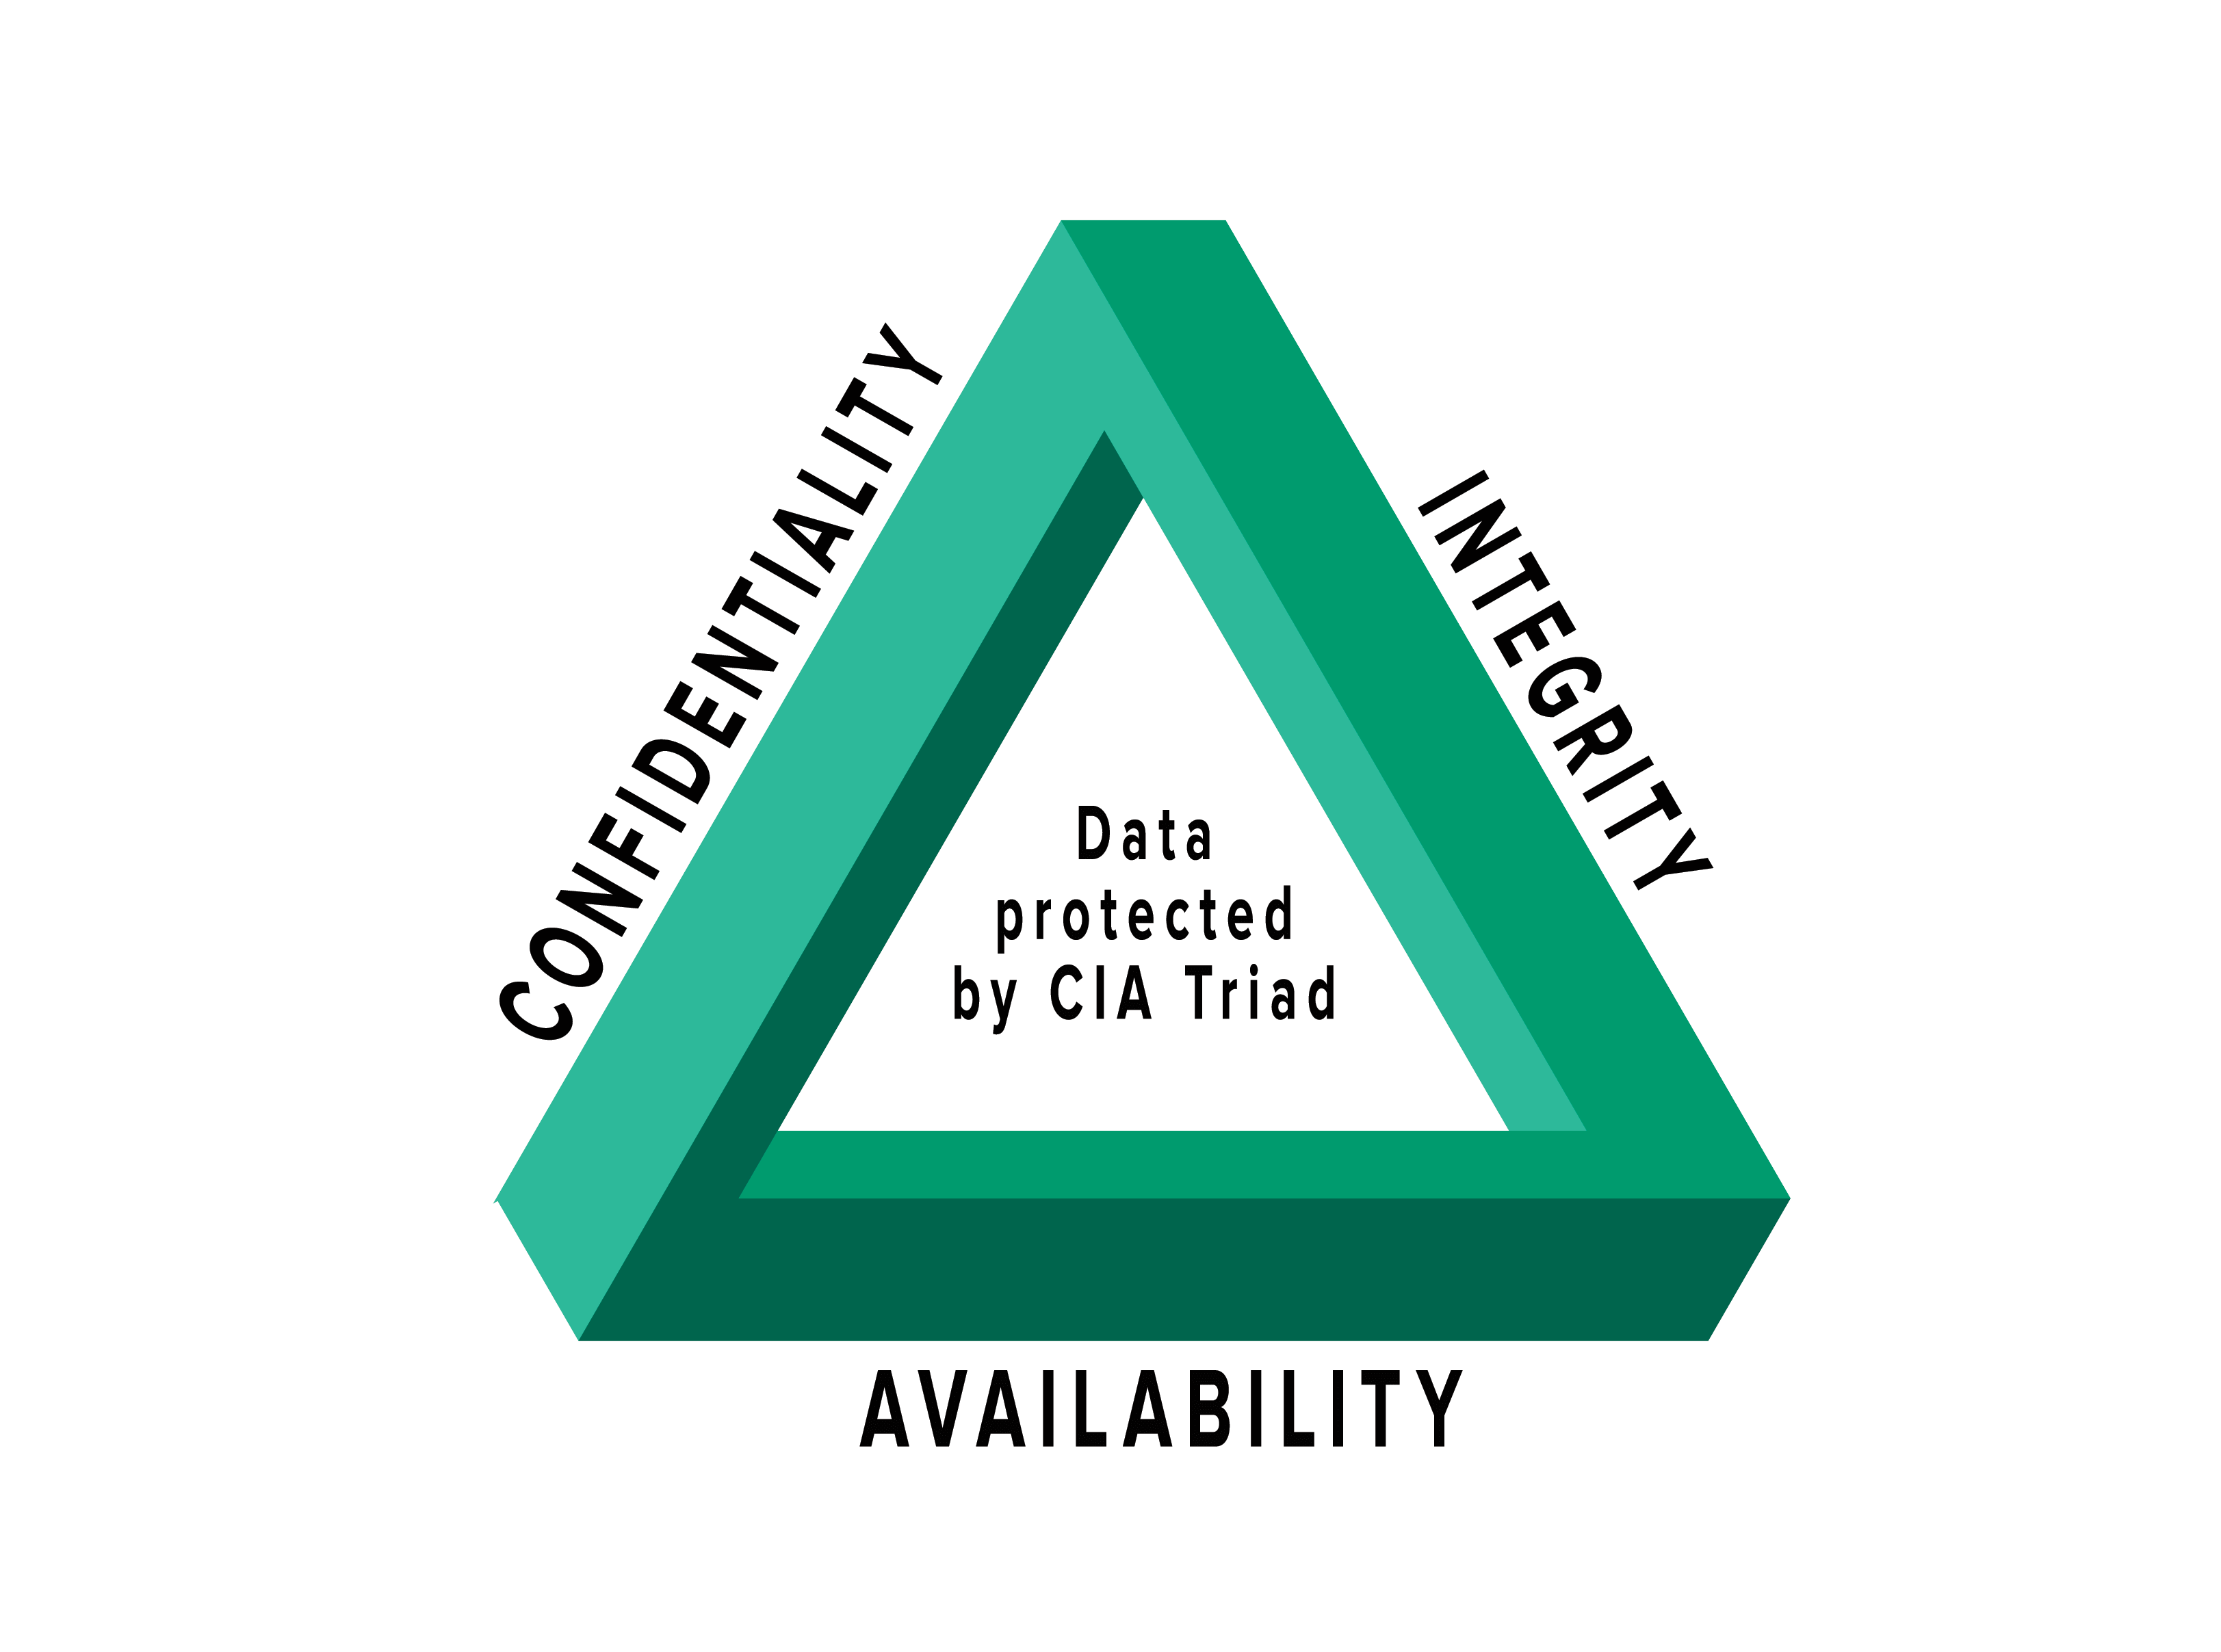
\includegraphics[width=\textwidth]{CIA TRIAD}
    \caption{CIA driehoek\autocite{Debbie2019} \label{fig:2.4}} 
    
\end{figure}
 
 Binnen IT-beveiliging is vertrouwelijkheid de top prioriteit, daaronder staat integriteit en als 3de beschikbaarheid~\autocite{Max2020}.
 
\subsubsection{\IfLanguageName{dutch}{Updates IT}{Updates IT}}
\label{subsec:Updates IT}
Updates binnen een IT-omgeving worden zo snel mogelijk uitgevoerd. Nieuwe updates zorgen voor een vermindering van kwetsbaarheden en oplossingen voor recente problemen. Een update zorgt voor een hogere vertrouwelijkheid wat het hoofddoel is van IT. Een kleine downtime bij een systeem maakt niet zoveel uit als bij een OT-omgeving~\autocite{Max2020}. 
\section{\IfLanguageName{dutch}{operationele technologie}{operationele technologie}}
\label{sec:operationele technologie}
\subsection{\IfLanguageName{dutch}{Definitie operationele technologie}{Definitie operationele technologie}}
\label{subsec:operationele technologie}
Operationele technologie (OT) verwijst volgens~\textcite{VirtualArmour2020} en~\textcite{Gartner} naar de hardware en software die binnen bedrijven wordt gebruikt om fysieke apparaten, processen en gebeurtenissen te wijzigen, bewaken of te controleren. Apparaten die zich bevinden in een OT-omgeving zijn meestal autonomer dan IT-apparaten. Velen gebruiken het woord industriële controle systemen (ICS) samen met operationele technologie of industriële technologie. ICS zijn controle netwerken en systemen om alle types van industriële processen te beveiligen. Het hoofddoel van operationele technologie en ICS is het optimaliseren van de industriële omgeving waarbij de machines continu kunnen draaien. Meestal wordt er gebruik gemaakt van volgende systemen binnen een OT-omgeving:
\begin{itemize}
    \item PLC (programmable logic controllers)
    \item RTU (remote terminal units)
    \item HMI (human machine interface)
    \item Historian
    \item SCADA (supervisory control and data acquisition)
    \item DCS (distributed control systems)
    
    
\end{itemize}
\subsection{\IfLanguageName{dutch}{Componenten}{Componenten}}
\label{subsec:OTcomponenten}
\subsubsection{\IfLanguageName{dutch}{PLC}{PLC}}
\label{subsubsec:PLC}
Volgens~\textcite{Unitronics} en~\textcite{2020} is een programmeerbare logische controller (PLC) een robuuste computer die wordt gebruikt voor industriële automatisering. De controllers kunnen een specifiek proces, machinefunctie of een hele productielijn automatiseren.

Een PLC ontvangt informatie die hij verwerft van sensoren of invoerapparaten die aangesloten zijn. Nadat de PLC de informatie heeft verwerkt zal hij uitgangen activeren op basis van voorgeprogrammeerde parameters. Een PLC kan tijdens de werking de gegevens die worden ingevoerd bewaken en registreren zoals bedrijfstemperatuur, processen starten en stoppen, alarmen, enzovoort. Een PLC kan op bijna elke toepassingen worden gebruikt.

Er zijn enkele componenten die een PLC onderscheiden van industriële computers, microcontrollers en andere industriële oplossingen wat u ook kan zien in figuur ~\ref{fig:2.5}.
\begin{itemize}
    \item I/O: De CPU van de PLC zal de data opslaan en verwerken binnen een gegeven tijd. De input en output modules daarnaast verbinden de PLC met de rest van de omgeving. De input module zal informatie leveren aan de CPU die deze informatie zal verwerken. Hierna zal de output module deze informatie doorsturen naar een ander component binnen het OT-netwerk. 
    \item Communicatie: PLC's hebben een aantal poorten en communicatieprotocollen die ervoor zorgen dat een PLC kan communiceren met andere systemen. Zo kan het zijn dat een PLC zijn data moet doorgeven aan een SCADA-systeem.
    \item HMI: Human machine interface(HMI) zijn computers die geconnecteerd zijn met PLC's of andere apparatuur in de OT-omgeving. Dit is een computer met een simpele display van wat de PLC doet. HMI's maken het makkelijk om informatie te lezen van de PLC's en eventueel zaken aan te passen indien nodig.
\end{itemize}
\begin{figure}
    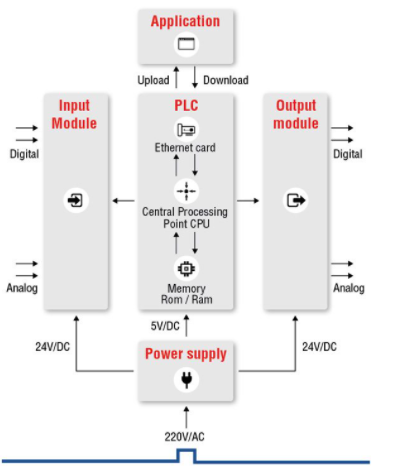
\includegraphics[width=\textwidth]{plc}
    \caption{Componenten van een PLC~\autocite{Unitronics} \label{fig:2.5}} 
\end{figure}


Tegenwoordig maken veel industriële omgevingen gebruik van all-in-once PLC's. Dit zijn PLC's met een geïntegreerd HMI-paneel. Het zorgt ervoor dat er maar 1 toestel moet geïnstalleerd worden wat tijdbesparend is, het vermindert bekabeling en tot slot vermindert het de kost van 2 toestellen te kopen.

Het programma dat wordt geïnstalleerd op de PLC's werd vroeger geschreven in 'Ladder Logic'. Dit is een programmeertaal die alles makkelijk visueel maakt en daardoor makkelijk is om te implementeren. Tegenwoordig wordt er meer gebruik gemaakt van C als programmeertaal voor PLC's.

Er zijn verschillende grote bedrijven die PLC's verdelen hieronder vind je enkele terug:
\begin{itemize}
    \item Siemens
    \item ABB
    \item Unitronics
\end{itemize}

\subsubsection{\IfLanguageName{dutch}{RTU}{RTU}}
\label{subsubsec:RTU}
Een Remote Terminal Unit (RTU), is een multifunctioneel apparaat bestaande uit een microprocessor die kan worden gebruikt voor het op afstand monitoren en beheren van diverse apparaten en systemen in de automatisering. Een RTU wordt normaal enkel ingezet in industriële omgevingen en lijkt op een PLC met het kleine verschil dat een RTU meer kan. Een RTU wordt meestal gekoppeld aan een SCADA-systeem~\autocite{Realpars2018}. 

Een RTU verschilt met een PLC op verschillende vlakken. Als eerste wordt een PLC gezien als een goedkoper alternatief, maar een RTU daarintegen is een meer robuuste toepassing. Dit zou er tot kunnen leiden dat een RTU langer meegaat en de iets duurdere kost zichzelf terug betaalt. Als tweede heeft een RTU enkele voordelen zoals back-up stroomopties en meer omgevingstolerantie dan de PLC. Ten derde heeft een PLC specifieke software nodig en het wordt geprogrammeerd in een specifieke taal 'ladder logic'. Een RTU wordt meestal geprogrammeerd in de vorm van een simpele web interface, die wordt meegeleverd met de RTU. Ook zijn er veel voorgeprogrammeerde modules die je enkel moet aanzetten bij een RTU wat zorgt voor weinig configuratie tijd. Enkele talen die bij een RTU gebruikt worden zijn: Basic, Visual Basic en C\#, maar ook ladder logic kan gebruikt worden. Tot slot is een groot voordeel van RTU's dat ze kunnen gebruikt worden in omgevingen met extreme temperaturen en plaatsen op een afstanden van kilometers lang. De RTU maakt communicatie mogelijk over vele kilometers en zal nooit uitvallen doordat ze meestal een back-up batterij hebben op zonne-energie. De nieuwe PLC's zorgen ervoor dat de meeste van deze verschillen kleiner worden, maar de omgeving factoren blijft het grote voordeel van de RTU~\autocite{Realpars2018}. In figuur ~\ref{fig:2.5} kan je zien welke modeleertalen er worden gebruikt voor een RTU, dat hij is verbonden met sensors van de industrie en hoe de RTU-verbinding maakt met een monitor via lange afstand.

\begin{figure}
    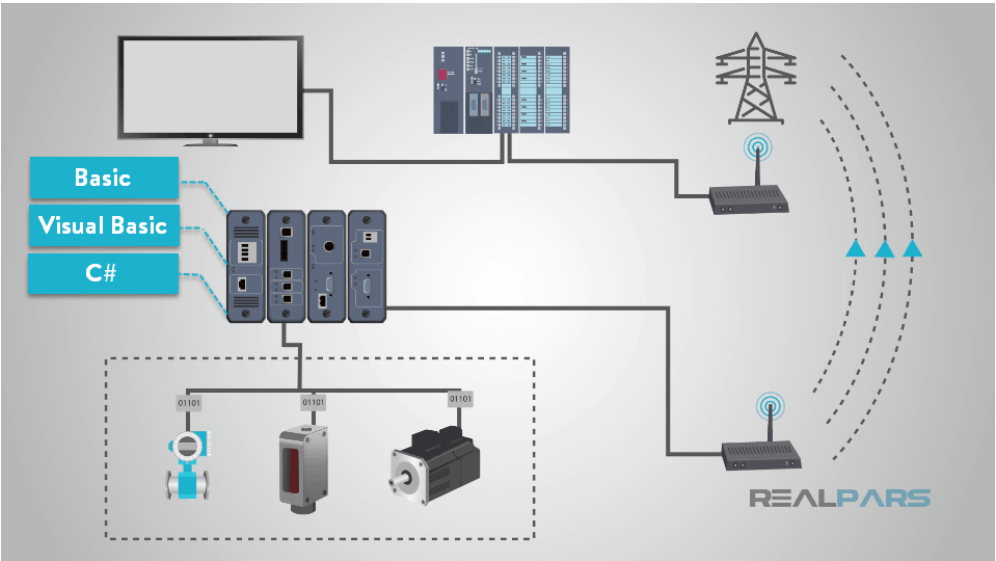
\includegraphics[width=\textwidth]{RTU}
    \caption{RTU modeleertalen en verbinding naar monitor~\autocite{Realpars2018} \label{fig:2.6}} 
\end{figure}

Er zijn verschillende grote bedrijven die PLC's verdelen hieronder vind je enkele terug:
\begin{itemize}
    \item Schneider Electric
    \item ABB
    \item Siemens Energy
\end{itemize}

\subsubsection{\IfLanguageName{dutch}{HMI}{HMI}}
\label{subsubsec:HMI}
Een Human machine interface (HMI) is een interface of dashboard dat een persoon connecteert met een machine, systeem of toestel. HMI's worden meestal gebruikt in industriële omgevingen waar ze instaan voor de controle en automatisatie van de machines. Een HMI kan verschillende vormen aannemen: een scherm op een machine, een tablet, een computer, druk-knop, en vele andere~\autocite{Exor2019} en~\autocite{2018}.

In industriële omgevingen heeft een HMI meerdere taken:
\begin{itemize}
    \item data visualiseren
    \item productietijd, trends en tags bijhouden
    \item input en output van machines monitoren
\end{itemize}

HMI's communiceren met Programmable Logic Controllers (PLC's) en input/output sensors om informatie te vergaren en te tonen. Ze kunnen gebruikt worden om belangrijke zaken van de productie te tonen, maar ook voor moeilijkere operaties zoals machines afsluiten en de productie snelheid veranderen. HMI's worden gebruikt om industriële processen te optimaliseren door gegevens te digitaliseren en te centraliseren. Door gebruik te maken van een HMI kunnen operatoren belangrijke informatie zien in grafieken of digitale dashboards, alarmen bekijken en beheren en verbinding maken met SCADA-systemen, allemaal via één console. Vroeger moesten werknemers elke keer gaan kijken naar vooruitgang van het systeem en dit noteren. Doordat PLC's nu real-time informatie kunnen doorsturen naar HMI's zijn deze werknemers niet meer nodig. Dit voorkomt het probleem van een menselijke fout of dat er te weinig informatie zichtbaar is~\autocite{2018}.


SCADA en HMI worden vaak in één context gebruikt maar er is weldegelijk een verschil tussen beide. HMI's zijn gericht op het visueel overbrengen van informatie om de gebruiker te helpen toezicht te houden op een industrieel proces. SCADA-systemen hebben een grotere capaciteit voor gegevensverzameling en bediening van het besturingssysteem. In tegenstelling tot SCADA-systemen  verzamelen en registreren HMI's geen informatie en maken ze geen verbinding met databanken. Een HMI is eerder een communicatiemiddel dat een functie heeft binnen een SCADA-systeem~\autocite{2018}.

Momenteel zijn er veel geavanceerde HMI's op de markt die bewaking en controle van fabrieksmachines mogelijk maken. De belangrijkste reden om te investeren in een geavanceerde HMI is de mogelijkheid om machines op afstand te monitoren en dashboards uit te voeren. Een ander voordeel is de mogelijkheid om realtime data te verkrijgen. Deze voordelen zorgen ervoor dat de complexiteit van een fabrieksomgeving vermindert. De geavanceerde HMI's zorgen ervoor dat eigenaren snel kunnen reageren op veranderde trends waardoor de tijd dat het niet optimaal werkt, wordt vermindert~\autocite{Exor2019}. 

HMI's worden door bijna alle industriële organisaties gebruikt. Enkele voorbeelden vindt u hieronder:~\autocite{2018}
\begin{itemize}
    \item Energie
    \item Transport
    \item water
\end{itemize}

\subsubsection{\IfLanguageName{dutch}{Historian}{Historian}}
\label{subsubsec:Historian}
Een historian server is een centraal punt voor het beheer, opslaan, comprimeren en opvragen van data die het verkrijgt van zijn verbonden apparaten via het netwerk. Alle data wordt opgeslagen in data archieven, waarbij elk archief een specifieke periode van historische gegevens bevat. Archieven en data kunnen verder opgesplitst worden in data stores. Dit is een logische verzameling van data die wordt gebruikt om data op te slaan, te organiseren en te beheren volgens de gegevensbron en de opslagvereisten. Het primaire gebruik van data stores scheidt verschillende soorten gegevens. Zo worden waarden die zelden veranderen in één data store gezet en andere data in een andere data store. Dit zal zorgen voor query performantie~\autocite{Solutions}.

Een historian kan berekeningen doen aan de hand van de data, en kan deze opslaan op de server in tags. Er bestaan ook server-to-server oplossingen die dezelfde berekeningen kunnen doen maar de berekende data versturen naar een remote server~\autocite{Solutions}. 

Volgens~\textcite{Rinaldi} zijn er echter veel verschillende types van historians die eindgebruikers kunnen gebruiken. Historians kunnen draaien in een PLC als applicatie, maar er kan ook een hele server worden opgezet die alle informatie van het netwerk zal verkrijgen. De historians kunnen ook onderverdeeld worden aan de hand van hoe ze data verkrijgen. Bij sommige servers wordt de data over het netwerk verkregen, maar vroeger gebruikten ze meestal USB's die ze om de zoveel tijd moesten gaan halen om de data over te zetten. Als laatste worden historians onderverdeeld aan de hand van hun functionaliteit. Simpele historians kunnen data verkrijgen en deze later doorsturen naar andere severs. Andere historians hebben ook datababank functionaliteiten die grafieken en analyses maken van de verkregen data.


\subsubsection{\IfLanguageName{dutch}{SCADA}{SCADA}}
\label{subsubsec:SCADA}

Supervisory control and data acquisition (SCADA) is een type van een controle proces systeem bestaande uit een softwaresysteem met hardware elementen om ervoor te zorgen dat industriële organistaties kunnen: 
\begin{itemize}
    \item Industriële processen lokaal of remote controleren en aanpassen
    \item Real-time data verkrijgen van de processen
    \item Direct reageren op toestellen door middel van een HMI
    \item Log files creëren van de toestellen
\end{itemize}
Een basis SCADA-)architectuur bestaat uit PLC's(~\ref{subsubsec:PLC}) of RTU's (~\ref{subsubsec:RTU}). Deze zullen communiceren met de HMI's, sensors, historian databanken en andere toestellen over het netwerk om alle informatie door te sturen naar een computer met SCADA-software op geïnstalleerd. De SCADA-software verwerkt en toont de data. Het SCADA-systeem zal de operatoren waarschuwen indien er iets fout gaat, waarna er dingen kunnen aangepast worden via de HMI. Een voorbeeld van een basis SCADA-architectuur vind je op figuur~\ref{fig:2.7}  ~\autocite{Muthukrishnan2021} en~\autocite{2018a}
\begin{figure}
    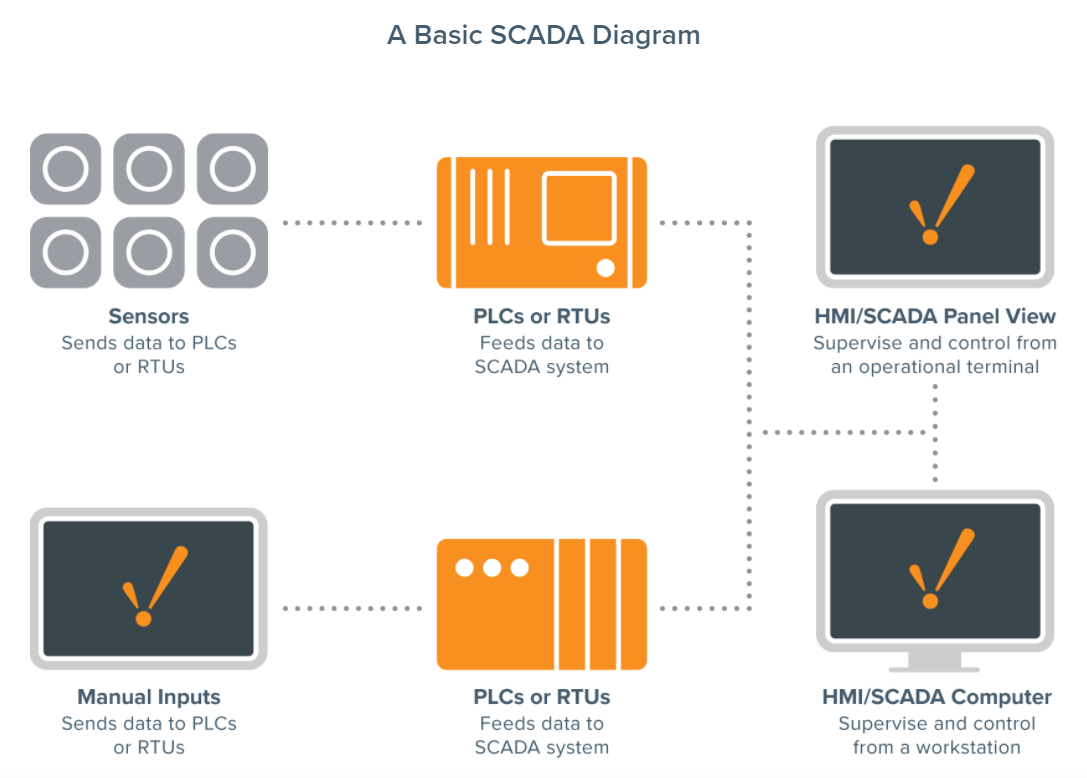
\includegraphics[width=\textwidth]{SCADA}
    \caption{Basis SCADA diagram~\autocite{2018a} \label{fig:2.7}} 
\end{figure}  

SCADA-systemen worden gebruikt in industriële omgevingen om efficiëntie te controleren, gegevens te distribueren en slimmere beslissingen te maken. Er zijn veel variaties mogelijk van SCADA-systemen, er zijn zowel eenvoudige als complexe installaties. Een SCADA-systeem is de ruggengraat van veel moderne OT-omgevingen, waaronder:~\autocite{Muthukrishnan2021} en~\autocite{2018a}
\begin{itemize}
    \item Energie.
    \item Voedsel.
    \item Transport.
    \item Olie en gas.
    \item En vele andere.
\end{itemize}

Vroeger was er veel personeel nodig om alle toestellen te monitoren en om ervoor te zorgen dat alles goed verliep. Het personeel moest elke keer op knoppen gaan drukken en kijken of er niets mis was met het systeem. Naarmate dat de industriële netwerken groter werden moesten er nieuwe oplossingen komen om deze gemakkelijk te monitoren en te beheren over een langere afstand. Rond 1970 kwam de term SCADA voor het eerst aan bod. In 1970 waren er nog geen netwerken zoals we deze vandaag kennen en waren de SCADA-systemen mainframe computers die volledig op zichzelf werkten. Vanaf de jaren 1990 en eerste jaren van de 21ste eeuw, is SCADA veel veranderd. Het ging van een systeem dat volledig op zichzelf werkte naar een systeem dat over het netwerk werkt met een heleboel andere systemen. Dit zorgde ervoor dat alle toestellen binnen het SCADA-systeem niet van één merk moest zijn~\autocite{Muthukrishnan2021} en~\autocite{2018a}.

Moderne SCADA-systemen beschikken over real-time data waardoor het makkelijk is om keuzes te maken om hun processen te verbeteren op elk moment. Invoering van moderne IT-componenten zoals SQL in SCADA-software heeft gezorgd voor een verbetering van efficiëntie, veiligheid, productiviteit en betrouwbaarheid van het systeem. Waar vroeger de databank van OT niet gekoppeld werd aan IT, is dit nu wel het geval met als voorbeeld SQL-databanken. Data dat wordt verzameld in OT kan makkelijk worden gekoppeld aan het ERP-systeem hierdoor~\autocite{2018a}.

\subsubsection{\IfLanguageName{dutch}{DCS}{DCS}}
\label{subsubsec:DCS}
Een distributed control system, ook wel DCS genoemd is een structuur dat wordt gebruikt binnen een operationeel netwerk om de verschillende processen van de fabriek te coördineren en te controleren~\autocite{Realpars2019}.

Vroeger toen de PLC net op de markt kwam, waren deze goed voor het bestuur van afzonderlijke processen en het gebruik in repetitieve en discrete besturing. De opkomst van de DCS was bedoeld voor besturing van veel autonome regelaars die veel continue processen afhandelden, voornamelijk met analoge besturing. De verschillen tussen een PLC en een DCS-systeem zijn over de jaren heen gebleven, zo zijn er nu nog altijd een paar essentiële verschillen~\autocite{Realpars2019}. 

PLC's worden voornamelijk gebruikt voor alleenstaande processen die snel bestuurbaar moeten zijn. Ze hebben een relatief eenvoudig, goedkoop ontwerp en vormen de kern van een OT-systeem. De verwerkingstijd van de taken van een PLC zijn heel snel, deze worden gecontroleerd door middel van een grafische display zoals SCADA~\autocite{Realpars2019}.

Een DCS wordt gebruikt voor continue, complexe besturingen en heeft een controlecentrum geïntegreerd in de software, zoals een SCADA, dat de kern van het systeem vormt. De verwerkingstijden van een DCS zijn iets trager en de beheerders communiceren met het besturingssysteem via grafische displays. Wanneer veiligheid een prioriteit is in een omgeving is een DCS een heel betrouwbaar systeem. Dit komt omdat de fabrikant zowel de besturing als de bewakingsapparatuur aanlevert in een geïntegreerd pakket, waardoor risico's van integratiefouten verminderen~\autocite{Realpars2019}.

Een DCS bestaat uit verschillende elementen. Als eerste zijn er beheerstations die het kloppend hart zijn van het DCS. Hier kunnen beheerders de fabriek observeren, de processen en alarmen nakijken, de productie monitoren en veel meer. Als tweede zijn er servers, archief en machine computers. De servers staan in voor de communicatie tussen de beheerstations en de processors in de fabriek. De archief computers staan in voor het bijhouden van historische data en de machine computers worden gebruikt om de processen aan te maken en te downloaden naar de processors. Als 3de component zijn er de DCS-controllers. Deze controleren alle processors individueel alsook de I/O modules. Een andere taak van deze controllers is het opleveren van data aan de servers om deze om te zetten naar grafische data. Dit gebeurt meestal aan de hand van industrieel ethernet of fiber optic. Als laatste zijn er de toestellen die worden gebruikt in de fabriek. Communicatie tussen deze toestellen en de processors kan heel gevarieerd zijn. Afhankelijk van het toestel kan gebruik worden gemaakt van industrieel ethernet, profibus DP, ethercat en vele andere protocollen die verder besproken zullen worden in dit hoofdstukcha. Toestellen op dit niveau zijn meestal, switches, motoren, zender, sensors en vele andere~\autocite{Realpars2019}.

\subsection{\IfLanguageName{dutch}{OT-protocollen}{OT-protocollen}}
\label{subsec:OT protocollen}
Uit onderzoek van~\textcite{Thomas2020} blijkt dat industrieel ethernet de leider is voor industriële communicatie die worden gebruikt binnen een industrieel netwerk, dit wordt ook weergegeven in figuur~\ref{fig:2.8}. Na ethernet komt fieldbus die lang op nummer één heeft gestaan en daarna komen de wireless protocollen. Industrieel ethernet stijgt elk jaar heel hard en heeft momenteel EtherNet/IP en profinet als twee grootste protocollen. Profibus is het grootste communicatieprotocol dat gebruikt wordt binnen fieldbus, maar ziet elk jaar een daling. Wireless staat al enkele jaren stabiel, maar hier wordt een toeneming voor verwacht binnen enkele jaren als 5G op zijn hoogtepunt komt. Aangezien momenteel EtherNet/IP en profinet de 2 grootste zijn zullen deze verder besproken worden. Andere protocollen die kunnen gebruikt worden binnen een industrieel netwerk zijn:
\begin{itemize}
    \item EtherCAT
    \item Modbus TCP
    \item POWERLINK
    \item CC-Link IE Field
    \item Bluetooth
    \item WLAN
    \item Profibus DP
    \item Modbus-RTU
    \item CC-Link
    \item CANopen
    \item DeviceNet
\end{itemize}
\begin{figure}
    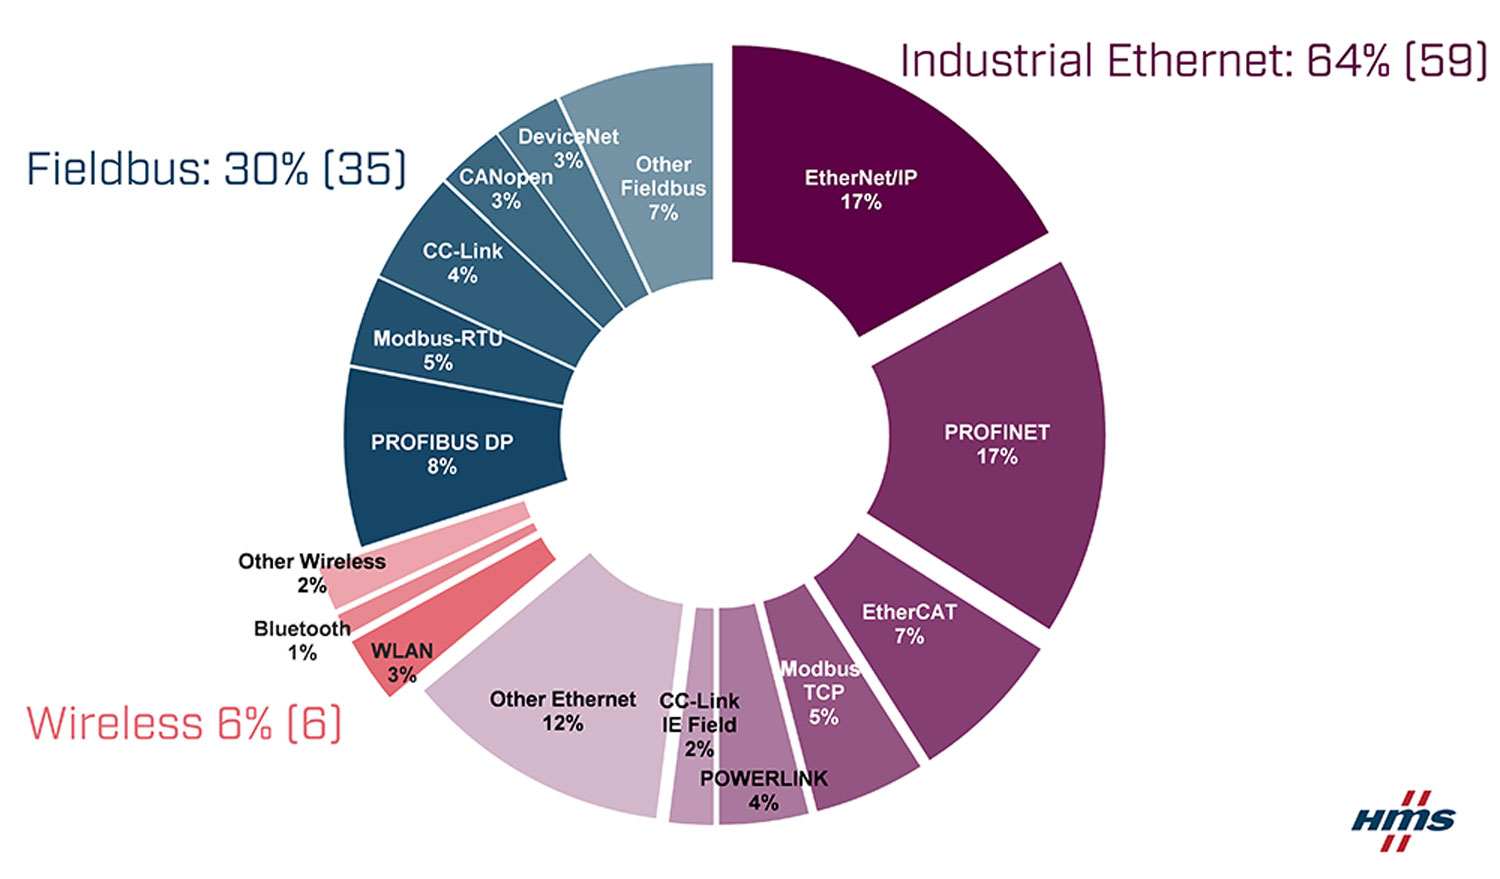
\includegraphics[width=\textwidth]{Protocollen OT}
    \caption{Protocollen OT~\autocite{Thomas2020} \label{fig:2.8}} 
\end{figure} 

\subsubsection{\IfLanguageName{dutch}{Industrieel ethernet}{Industrieel ethernet}}
\label{subsubsec:Industrieel ethernet}
Industrieel ethernet en gewoon ethernet dat wordt gebruikt in kantooromgevingen zijn niet helemaal hetzelfde. Er zijn enkele gelijkenissen maar ook verschillen~\autocite{Tannehill2020}.

Aangezien industrieel ethernet en gewoon ethernet uit dezelfde basis zijn opgebouwd zijn ze op enkele vlakken hetzelfde. Als eerste hebben ze een aantal gemeenschappelijke communicatiekenmerken, zoals de framegrootte en signaalniveaus. Ten tweede bieden beide soorten verschillende datatransmissiesnelheden van 10 Mbps tot 1 Gbps en meer. 100 Mbps is een gebruikelijke snelheid voor industriële toepassingen. Commercieel ethernet maakt meestal gebruik van hogere transmissiesnelheden om de communicatie van streaming en video aan te kunnen bieden. Ten derde maken beide gebruik van verschillende categorieën ethernet-kabels, afhankelijk van de netwerkkenmerken~\autocite{Tannehill2020}.

De belangrijkste verschillen tussen commercieel ethernet en industrieel ethernet komen neer op vereisten en bedrijfsomstandigheden. Ten eerste wordt industrieel ethernet gebruikt voor kritische doeleinden. Het is de bedoeling dat downtime van processen zoveel mogelijk wordt vermeden. Als dit niet het geval is kan dit een grote impact hebben op het bedrijfsresultaat. Wanneer in een industrieel ethernet netwerk blijkt dat een pakket niet is aangekomen, wordt dit opnieuw verzonden. Als een pakket niet toekomt in een commercieel netwerk is dit niet heel erg. Ten tweede zijn de omgevingsfactoren binnen een industrieel netwerk helemaal anders dan in een commercieel netwerk. Ethernet dat wordt gebruikt in een industrieel netwerk moet bestend zijn tegen lawaai, hoge of lage temperaturen, schokken en dergelijke. Als laatste moet elektromagnetische ruis vermeden worden binnen een industrieel netwerk. Doordat in een fabriek veel installaties en toepassingen staan is er een stroom aan magnetische, radiofrequentie-interferentie en elektrostatische ruis. Als deze ruis een ethernet pakket aanraakt kan het zijn dat het hele pakket geweigerd wordt door het apparaat~\autocite{Tannehill2020}.

\subsubsection{\IfLanguageName{dutch}{Verschil ethernet en fieldbus}{Verschil ethernet en fieldbus}}
\label{subsubsec:Verschil ethernet en fieldbus+}
Ethernet en fieldbus hebben hetzelfde doel voor ogen, namelijk communicatie verzorgen tussen industriële machines. Fieldbus is een manier om een netwerk van productieapparatuur in real-time te verbinden en te besturen. Waar vroeger altijd een point-to-point verbinding werd gebruikt is dit verandert naar één digitale verbinding waarop alle informatie in serie wordt overgedragen. De apparaten worden in een fieldbus omgeving verbonden met elkaar door een kabel en communiceren via desbetreffende fieldbus protocollen. Zoals reeds aangehaald in \ref{subsec:OT protocollen} is ethernet aan het stijgen tegenover fieldbus. Er zijn enkele verschillen tussen beide die hiervoor zorgen. Industrieel ethernet biedt hogere snelheden, een grotere verbindingsafstand en de mogelijkheid om meer apparaten aan te sluiten. Standaard ethernet protocollen kunnen een lage latency bereiken en maken een flexibele netwerktopologie mogelijk. Ook is de real-time nauwkeurigheid beter bij ethernet protocollen. Als laatste zijn de fieldbus componenten duurder dan die van ethernet~\autocite{Chemigraphic2019}.



\subsubsection{\IfLanguageName{dutch}{Profinet}{Profinet}}
\label{subsubsec:Profinet}
Profinet is een open industriële ethernet-oplossing op basis van normen die internationaal worden vastgelegd. Het is een communicatieprotocol dat is gemaakt voor de gegevensuitwisseling tussen controllers en andere apparaten die zich bevinden in de automatiseringomgeving. Rond de jaren 2000 is het protocol geïntroduceerd en sindsdien is het één van de meest toegepaste oplossing voor industrieel ethernet. Aangezien het een open standaard is, zijn er veel producten zoals PLC's ontwikkeld speciaal voor profinet~\autocite{Nelly2021}.

Om alle componenten van een industriële omgeving met elkaar te verbinden maakt profinet gebruik van de standaard ethernet als communicatiemedium. Ethernetkabels verbinden profinet componenten binnen een netwerk waardoor ook andere ethernet protocollen kunnen gebruikt worden binnen het netwerk zoals HTTP~\autocite{Nelly2021}.

Industriële automatiseringsomgevingen vereisen meestal een hoge snelheid en een communicatie waar berichten precies worden afgeleverd wanneer het verwacht wordt. Profinet zal ervoor moeten zorgen dat de snelheid optimaal is afhankelijk van de taak. Er zijn taken zoals het laden van configuratiegegevens die enkele minuten mogen duren, maar communicatievertraging van slechts enkele miliseconden tussen een PLC en een motor die het systeem aanstuurt kan het proces aanzienlijk beïnvloeden. Om een goede prestatie te leveren biedt profinet gegevens aan via volgende communicatiekanalen:
\begin{itemize}
    \item TCP/IP (of UDP/IP)
    \item Profinet Real-Time (RT)
    \item Profinet isochrone Real-Time(IRT)
    \item Tijdgevoelige netwerken (TSN)
\end{itemize}
Voor processen die niet tijdkritisch zijn kan profinet gebruik maken van TCP/IP of UDP/IP-communicatie. Deze communicatie is echter niet goed voor tijdkrische taken. Hiervoor kan profinet gebruik maken van een real-time kanaal om gegevens snel te leveren~\autocite{Nelly2021}.

Profinet real-time maakt gebruik van een standaard ethernet frame dat een ethertype bevat. Profinet real-time communicatie ethertype is ingesteld op 0x8892. Bij aankomst op het bestemmingspunt wordt het frame onmiddelijk naar de profinet toepassing geleid. De data gaat direct van laag twee naar laag zeven. Hierdoor worden de TCP/IP-lagen overgeslagen en wordt de variabele tijd vermeden. De communicatiesnelheid verbeterd hierdoor aanzienlijk~\autocite{Nelly2021}.

Zoals reeds aangetoond is, voldoet profinet real-time aan de meeste eisen van tijdkritische toepassingen. Er is geen speciale hardware of configuratie nodig om het real-time mechanisme van profinet te gebruiken aangezien dit standaard in de profinet-producten zit~\autocite{Nelly2021}.

\subsubsection{\IfLanguageName{dutch}{Ethernet/IP}{Ethernet/IP}}
\label{subsubsec:EtherNet/IP}
Ethernet in ethernet/IP is een protocol dat elke dag wordt gebruikt door heel veel mensen. De communicatie tussen computers verloopt over netwerken via paketten. Aangezien veel computers data willen verzenden, zijn er enkele regels opgesteld voor het verzenden en krijgen van pakketten~\autocite{Realpars2019a}. 

Ethernet maakt gebruik van het TCP/IP-model. Dit protocol wordt gebruikt voor communicatie over het internet. TCP staat voor `Transmission Control Protocol` en IP staat voor `Internet Protocol`. Het TCP/IP-protocol bestaat uit 4 lagen: Applicatie, TCP, IP en netwerk laag, zoals je kan zien in figuur~\ref{fig:2.10}. Elke laag heeft zijn eigen functie en als deze zijn functie gedaan heeft wordt het doorgestuurd naar de volgende laag. Een computer zal zijn data doorsturen naar de applicatie laag. Deze laag zal data over de applicatie toevoegen die nodig is en daarna doorsturen naar de TCP laag. De TCP laag zal de data uitpakken en kijken of er fouten inzitten. Hierna zal hij de data doorsturen naar de IP laag. De IP laag zal specifieke data toevoegen voor dat pakket. De netwerk laag zal de data omvormen naar een Ethernet pakket of ander pakket naargelang de communicatie. Dit pakket zal altijd door deze 4 lagen gaan om het einddoel te bereiken. Het einddoel kan niet enkel een computer zijn, maar ook andere netwerkcomponenten zoals een PLC~\autocite{Realpars2019a}.
\begin{figure}
    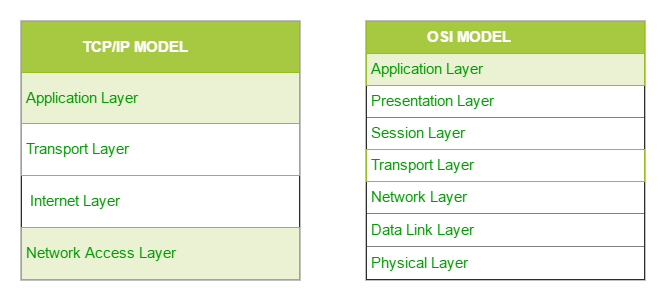
\includegraphics[width=\textwidth]{TCPIP}
    \caption{TCP/IP-model\autocite{GeeksforGeeks2020a} \label{fig:2.9}} 
    
\end{figure}

IP in ethernet/IP staat voor industrieel protocol. Dit betekent dat ethernet wordt gebruikt in combinatie met het industrieel protocol dat gebruik maakt van CIP-lagen (Common Industrial Protocol) gecombineerd met de TCP/IP of UDP-lagen om een protocol te creëren dat kan worden gebruikt voor gegevensuitwisseling en controletoepassingen. In figuur~\ref{fig:2.10} is het OSI-model uitgelegd aan de hand van het industrieel ethernet/IP-protocol. Bij het TCP/IP-protocol zal er een bericht worden gestuurd en als deze goed is aangekomen zal er een bericht terug worden gestuurd. Dit soort protocol wordt gebruikt als er een snelheid moet bereikt worden. Het UDP/IP-protocol hoeft geen bericht terug te krijgen. Dit wordt gebruikt op PLC's of apparaten die constant de staat van hun data doorsturen. Als er een pakketje niet bereikt is, geeft dit niet veel fouten. CIP maakt gebruik van een objectgeoriënteerd ontwerp om zaken te presenteren. Dit soort bericht kan worden gebruikt bij PLC-apparaten en toont aan welke gegevens gebruikt worden, bv snelheid, storingen of frequentie~\autocite{Realpars2019a}.
\begin{figure} 
    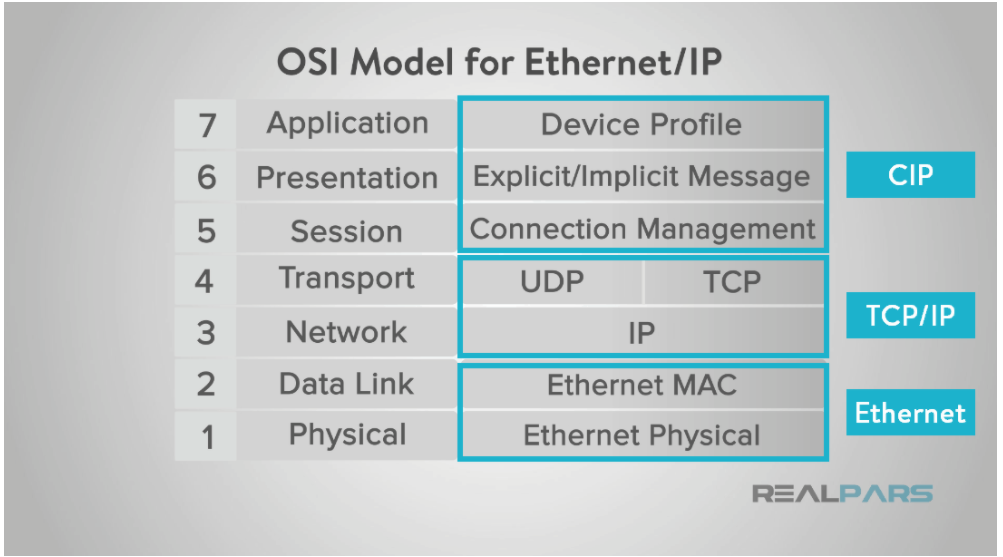
\includegraphics[width=\textwidth]{EthernetIP}
    \caption{OSI-model voor ethernet/IP\autocite{Realpars2019a} \label{fig:2.10}} 
\end{figure}

Het ethernet/IP-protocol is compatibel met veel standaard-switches die in de industriële omgeving worden gebruikt, waardoor het makkelijk te implementeren is. Snelheden van 10 of 100mbps kunnen makkelijk verwerkt worden met deze switches. In de eenvoudigste bewoordingen zijn Ethernet/IP Ethernet-pakketten die worden gebruikt met het industriële protocol van CIP, TCP/IP, en/of UDP-lagen om de vereiste gegevens aan uw controller te leveren~\autocite{Realpars2019a}.

\subsection{\IfLanguageName{dutch}{OT-security}{OT-security}}
\label{subsec:OT security}
\subsubsection{\IfLanguageName{dutch}{Wat valt er onder OT-security?}{Wat valt er onder OT-security?}}
\label{subsec:Wat valt er onder OT security?}
Volgens~\textcite{Infradata2019} is OT-beveiliging alle hardware en software dat wordt gebruikt om veranderingen in apparaten, processen en gebeurtenissen te bewaken, te detecteren en te controleren. OT-beveiliging wordt gebruikt om industriële systemen en netwerken te beschermen tegen interne en externe aanvallen. 

OT-systemen werden vroeger helemaal afgescheiden opgezet van het IT-netwerk. Er waren vrijwel geen aanvallen op de OT-systemen, omdat het moeilijk was binnen te geraken. Enkel interne aanvallen waren onvermijdelijk. Sinds de convergentie van IT en OT-netwerken hebben aanvallers hun zinnen gezet op het inbreken in OT-netwerken. Meestal kunnen hackers via het IT-netwerk, het OT-netwerk infecteren. Enkele aanvallen die de dag van vandaag worden gebruikt binnen OT-netwerken zijn:
\begin{itemize}
    \item Ransomware
    \item Malware
    \item Human error
    \item Ddos en botnet aanvallen
\end{itemize}
Belangrijke factoren voor bedrijven die hun industriële netwerken willen beveiligen, zijn de hoge kosten van de apparatuur en de verwoesting die een aanval kan aanrichten. De nieuwe IT-trends en innovaties hebben een grote invloed op OT gebied. Industriële IoT toestellen leiden tot meer connectiviteit met de buitenwereld. Door deze toenemende connectiviteit nemen de veiligheidsrisico's toe~\autocite{Infradata2019} en~\autocite{Security2020}.

SCADA en industriële controlesystemen worden meestal gebruikt binnen OT-beveiliging. SCADA-beveiliging zorgt voor beveiliging van netwerken voor toezicht, controle en gegevensverwerking. Dit is een controlesysteem die bij industriële netwerken wordt gebruikt. Industriële contorlesystemen zijn toepassingen met een hoge beschikbaarheid. Deze systemen worden gebruikt om industriële processen te controleren en te bewaken. Een voorbeeld van een industrieel controlesysteem zijn alameren van gebouwinformatiesystemen~\autocite{Infradata2019}.


Net zoals bij IT-beveiliging moeten de werknemers binnen een industriële omgeving goed geïnformeerd zijn in verband met beveiliging. Vele malware bestanden komen binnen via mail. Dit kan voorkomen worden door de werknemers een uitgebreide training te geven in verband met beveiliging~\autocite{Infradata2019} en~\autocite{Security2020}.

Het beveiligen van een OT-omgeving wordt gedaan door netwerkbeveiliging en endpointbeveiliging. Netwerkbeveiliging bestaat uit tools om het netwerk te monitoren en te analyseren. Een bekend voorbeeld hierbij is de fortigate next generation firewall van Fortinet. Deze biedt een gecentraliseerd beheer over de industriële omgeving waarbij alles wordt gemonitord en geanalyseerd. Zo een firewall doet niet enkel aan netwerkbeveiliging maar ook aan internetbeveiliging aangezien het alles nakijkt van verkeer dat via het internet binnenkomt. Naast de netwerkbeveiliging kan endpointbeveiliging worden geïnstalleerd op toestellen binnen de industriële omgeving. Endpointbeveiliging beschermt componenten tegen: malware, illegale software en ongeautoriseerde apparaat verbindingen. Deze vorm van bescherming kan meestal zowel lokaal als vanop afstand worden beheert~\autocite{Infradata2019} en~\autocite{Security2020}.

\subsubsection{\IfLanguageName{dutch}{AIC-driehoek}{AIC-driehoek}}
\label{subsec:AIC driehoek}
De CIA-driehoek die uitgelegd staat in~\ref{subsec:CIA driehoek} kan ook gebruikt worden in OT-omgevingen. Hier wordt het in plaats van CIA-driehoek, de AIC-driehoek. Dit komt omdat beschikbaarheid van industriële processen de top prioriteit is binnen industrële omgevingen. Op de 2de plaats komt integriteit en als 3de vertrouwelijkheid~\autocite{Max2020}.   
\subsubsection{\IfLanguageName{dutch}{Updates OT}{Updates OT}}
\label{subsec:Updates OT}
Updates binnen een OT-netwerk zijn verschillend van updates binnen een IT-netwerk. In een OT-netwerk worden updates meestal niet direct uitgevoerd, omdat er in het begin nog fouten inzitten. OT hun doel is om zo weinig mogelijk downtime te hebben en een update zou dit kunnen verstoren. Er zijn industriële omgevingen waar er al enkele jaren geen updates zijn uitgevoerd en op de eerste versies blijven werken om downtime te voorkomen. Echter zijn dit soort omgevingen aan het verdwijnen en wordt de tijd tussen updates minder voor beveiligingsredenen~\autocite{Max2020}.
\section{\IfLanguageName{dutch}{Vergelijking IT en OT}{Vergelijking IT en OT}}
\label{sec:Vergelijking IT en OT}
Uit vorige hoofdstukken kunnen we afleiden dat er enkele verschillen en gelijkenissen zijn tussen een IT en OT-omgeving. De grote verschillen worden in het kort aangekaart in figuur~\ref{fig:2.11}. Dit is dan ook een antwoord op een deel van de hoofdonderzoeksvraag te vinden in sectie~\ref{subsec:hoofdonderzoeksvraag} en op enkele deelvragen die te vinden zijn in sectie~\ref{subsec:deelonderzoeksvraag}.

Als we kijken naar de componenten van beide omgevingen zien we een duidelijk verschil. In een IT-omgeving wordt er gebruik gemaakt van verschillende servers die nodig zijn voor de dagelijkse werking van een kantooromgeving. Zo zien we dat er bestandsservers, mailservers, webservers en andere worden gebruikt. Binnen een OT-omgeving wordt er vooral gebruik gemaakt van componenten om machines aan te sturen, zoals een PLC of RTU. Echter zijn er ook gelijkenissen tussen beide omgevingen. Een DHCP-server die typisch in een IT-omgeving staat kan ook worden gebruikt binnen een OT-omgeving. Toen IT en OT nog volledig gescheiden van elkaar werden opgezet werd dit niet gebruikt binnen een OT-omgeving, maar sinds de convergentie wordt de DHCP-server van de IT-omgeving meer en meer gebruikt om OT-componenten een IP-adres te geven. Een bestandsserver die in een IT-omgeving staat wordt in een OT-omgeving vervangen door een historian. Ze hebben dezelfde taak, elk binnen hun eigen omgeving. 

De protocollen binnen beide netwerken verschillen van elkaar, maar groeien steeds meer naar elkaar toe. In een IT-netwerk wordt vooral gebruik gemaakt van het TCP/IP-protocol om berichten te versturen over het internet. Dit is een algemene regel die alle toestellen gebruiken. Binnen een OT-omgeving is dit anders. Vroeger leverden veel hardware verkopers hun eigen protocollen bij hun componenten. Dit zorgde ervoor dat componenten van verschillende verkopers niet met elkaar konden communiceren. Nieuwe protocollen die worden gebruikt zoals ethernet/IP maken gebruik van het TCP/IP-model. Dit zorgt ervoor dat alles makkelijk te versturen is en dat elk toestel het kan ontvangen.

Beveiliging tussen de IT en OT-omgeving kent enkele verschillen en enkele gelijkenissen. Binnen de IT-omgeving wordt ingezet op applicatiebeveiliging en cloudbeveiliging, dit gebeurt niet binnen een OT-omgeving, omdat dit niet in een OT-omgeving past. De frequentie van updates is ook verschillend tussen beide omgevingen. Binnen een IT-omgeving worden updates vrij snel ingevoerd, in een OT-omgeving gebeurt dit minder snel of helemaal niet. Binnen de IT-omgeving moet vertrouwelijkheid van data altijd voorop gesteld worden, binnen een OT-omgeving is de beschikbaarheid van de processen de hoogste prioriteit. Naast al deze verschillen zijn er ook enkele gelijkenissen, zo wordt er binnen beide omgevingen gebruik gemaakt van netwerkbeveiliging, internetbeveiliging en endpointbeveiliging. 
\begin{figure}
    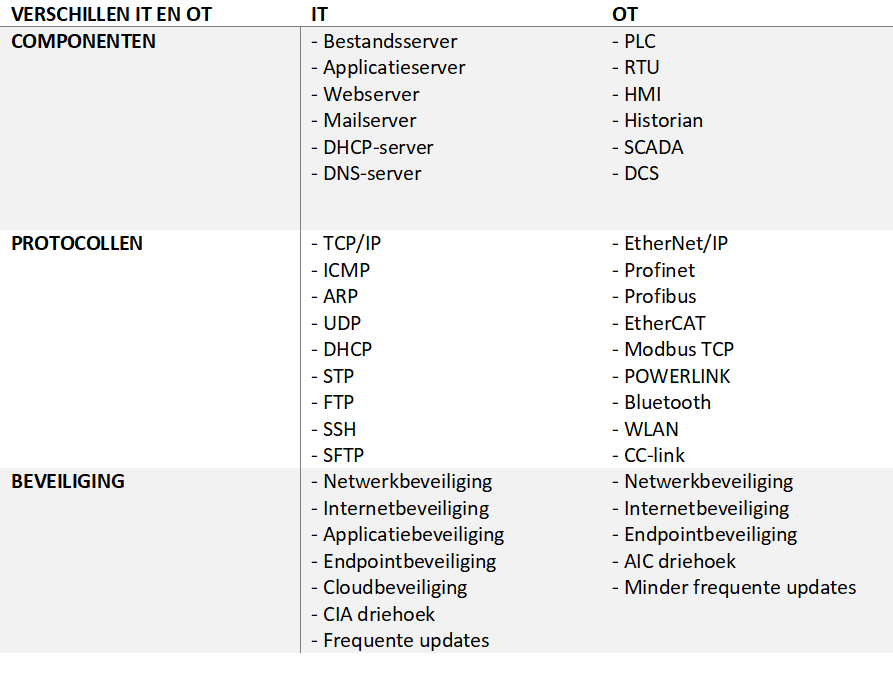
\includegraphics[width=\textwidth]{Verschillen IT en OT}
    \caption{Verschillen IT en OT \label{fig:2.11}} 
\end{figure}
\section{\IfLanguageName{dutch}{Convergentie IT en OT}{Convergentie IT en OT}}
\label{sec:Convergentie IT en OT}
In het begin van IT en OT werden beide omgevingen volledig afgescheiden van elkaar opgezet. Dit was, omdat beide omgevingen totaal verschillende doelen hadden vroeger. IT stond in voor gegevensopslag, ERP, Customer Relationship Management (CRM) en andere IT-systemen die we de dag van vandaag kennen. OT stond in voor het uitvoeren van fysieke processen. Naast de verschillende doelen waren deze vroeger ook niet ontworpen om samen te werken. Zo werden er totaal verschillende protocollen gebruikt binnen elke omgeving wat ervoor zorgde dat communicatie tussen beide omgevingen onmogelijk was. Deze integratie-uitdagingen, samen met beveiligingsproblemen, hoge aanloopkosten, IIoT-connectiviteitsproblemen en andere uitdagingen hebben ertoe bijgedragen dat IT en OT-systemen lang gescheiden van elkaar zijn gebleven~\autocite{Remy2020} en ~\autocite{SecureiconTeam2019}.

Sinds enkele jaren geleden is de convergentie van beide omgevingen gestart. De IT/OT-convergentie verbindt IT-systemen met OT-systemen waardoor ze gegevens makkelijk naar elkaar kunnen doorsturen. Het doel van de convergentie is om deze connectiviteit te gebruiken om de waarde van de systemen te verhogen. Veel bedrijven convergeren IT met OT om OT-gegevens te gebruiken met als doel IT-systemen te verbeteren of waardevolle inzichten te genereren. Ook worden de IT-gegevens gebruikt om OT-systemen te verbeteren, zodat fysieke operaties beter kunnen uitgevoerd worden~\autocite{Remy2020} en ~\autocite{SecureiconTeam2019}. 

De IT/OT-convergentie brengt enkele voordelen met zich mee, anders zou de convergentie compleet nutteloos zijn. Deze voordelen zijn voor de meeste bedrijven hun drijfveer om de convergentie te laten plaatsvinden. Dit is dan ook een antwoord op een deel van de hoofdonderzoeksvraag te vinden in~\ref{subsec:hoofdonderzoeksvraag}.
\begin{itemize}
    \item Minder downtime en lagere onderhoudskosten: OT-gegevens van apparatuur kunnen verzamelt en vervolgens geanalyseerd worden door de IT-systemen om te bepalen wanneer apparatuur onderhoud nodig zal hebben. Ook het onderhoud kan op afstand worden uitgevoerd door de apparaten die de informatie verzamelen. Dit zorgt voor een verminderde kost voor het bedrijf. Als er echter effectief zaken moeten gerepareerd worden zal er een werknemer nodig zijn die dit doet.
    \item Verbeterde innovatie: Door OT-gegevens te verzamelen van de klanten hun apparatuur kan worden bekeken hoe deze apparatuur wordt gebruikt op dagelijkse basis. Na het analyseren van deze gegevens kan dit nieuwe inzichten genereren over welke soorten innovaties de meeste waarde zouden leveren voor hun klanten. 
    \item Real-time data analyse.
\end{itemize}

Naast de voordelen zorgt de convergentie ook voor enkele nadelen.
\begin{itemize}
    \item OT wordt kwetsbaar voor dezelfde aanvallen die ze gebruiken binnen IT: Wanneer het IT en het OT netwerk worden geconnecteerd zal er data van het IT-netwerk naar het OT-netwerk verstuurd kunnen worden. Dit betekent dat als een hacker binnen geraakt in een IT-netwerk het ook in het OT-netwerk kan komen als dit niet goed beveiligd is. Vroeger werd OT-beveiliging niet of weinig toegepast. IT-managers moeten rekening houden dat bij de convergentie ook extra beveiliging komt kijken. 
    \item Verschillende communicatieprotocollen: Het is voor bedrijven niet gemakkelijk om data te verzamelen van OT-componenten, omdat deze andere communicatieprotocollen gebruikt dan IT-toestellen.
\end{itemize}

\subsection{\IfLanguageName{dutch}{Nieuwe begrippen leiden tot de convergentie}{Nieuwe begrippen leiden tot de convergentie}}
\label{sec:Nieuwe begrippen leiden tot de convergentie}
Nieuwe begrippen zoals de internet of things (IOT) en big data hebben een invloed op de convergentie van de IT en OT-omgeving. Meer en meer organisaties maken de dag van vandaag gebruik van industriële internet of things (IIoT) technologieën, zoals slimme meters, sensors en zelfcontrolerende transformatoren in hun productielijnen. De opkomst van deze nieuwe technologieën heeft een behoefte gecreëerd voor organisaties om te optimaliseren hoe machines, applicaties en infrastructuur gegevens verzamelen, verzenden en verwerken. De grote hoeveelheid gegevens die wordt gecreëerd moet worden verspreid en bijgehouden over verschillende locaties. Deze data is niet langer meer kleinschalig, maar door de sensors wordt zoveel data verstuurd dat het begrip big data wordt gebruikt. Dit is een grote hoeveelheid gegevens die te groot wordt voor een regulier databasemanagementsysteem. De IT/OT-convergentie geeft een sterke basis voor het gebruik van deze data om interne processen en zakelijke beslissen uit te voeren~\autocite{Tiempo2020}.

